%%%%%%%%%%%%%%%%%%%%%%%%%%%%%%%%% author.tex %%%%%%%%%%%%%%%%%%%%%%%%%%%%%%%%%
%
% sample root file for your "contribution" to a contributed volume
%
% Use this file as a template for your own input.
%
%%%%%%%%%%%%%%%%%%%%%%%%%%%%%%%%%% Springer %%%%%%%%%%%%%%%%%%%%%%%%%%%%%%%%%%



% RECOMMENDED %%%%%%%%%%%%%%%%%%%%%%%%%%%%%%%%%%%%%%%%%%%%%%%%%%%%%%%%%%%%%%%%
\documentclass[graybox]{svmult}

% choose options for [] as required from the list
% in the Reference Guide

\usepackage{mathptmx}           % selects Times Roman as basic font
\usepackage{helvet}             % selects Helvetica as sans-serif font
\usepackage{courier}            % selects Courier as typewriter font
\usepackage{type1cm}            % activate if the above 3 fonts are
                                % not available on your system

%\usepackage{makeidx}            % allows index generation
%\usepackage[dvips]{graphicx}
%\usepackage[dvipdfmx]{graphicx}
\usepackage{graphicx}           % standard LaTeX graphics tool when including figure files

%\usepackage{subfig}
\usepackage{subfigure}
\usepackage{algorithmic}
\usepackage{algorithm}
\usepackage{cite}


%\usepackage{multicol}           % used for the two-column index
%\usepackage[bottom]{footmisc}   % places footnotes at page bottom
\usepackage{booktabs} 
\usepackage{arydshln}
%\usepackage{natbib}
%\usepackage[numbers]{natbib}
%\usepackage[round]{natbib}
%\usepackage[numbers,sort&compress]{natbib}
%\bibliographystyle{unsrtnat}
%\usepackage[numbers,sort&compress]{natbib}
\usepackage{svg}
\usepackage{float}
\usepackage{newtxtext,newtxmath} %これで英文字も綺麗なベクターになる(timesより優秀)
\def\vector#1{\mbox{\boldmath $#1$}}



% see the list of further useful packages
% in the Reference Guide

\makeindex             % used for the subject index
                       % please use the style svind.ist with
                       % your makeindex program


%%%%%%%%%%%%%%%%%%%%%%%%%%%%%%%%%%%%%%%%%%%%%%%%%%%%%%%%%%%%%%%%%%%%%%%%%%%%%%

\begin{document}
\title*{Wearable Haptic Feedback Glove for Texture Rendering in Virtual Reality}

% Use \titlerunning{Short Title} for an abbreviated version of
% your contribution title if the original one is too long
\titlerunning{Wearable Haptic Feedback Glove for Texture Rendering in Virtual Reality}

\author{Korntawat Witchuvanit, Makio Ishihara}

% Use \authorrunning{Short Title} for an abbreviated version of
% your contribution title if the original one is too long
\authorrunning{K. Witchuvanit, M. Ishihara}

\institute{
	Korntawat Witchuvanit
	\at Graduate School of Engineering, Fukuoka Institute of Technology,\\
	3-30-1 Wajiro-Higashi, Higashi-Ku, Fukuoka 811-0295, Japan,\\ 
	\email{mfm23201@bene.fit.ac.jp}
	\and 
	Makio Ishihara 
	\at Department of Information and Communication Engineering, Fukuoka Institute of Technology,\\
	3-30-1 Wajiro-Higashi, Higashi-Ku, Fukuoka 811-0295, Japan,\\ 
	\email{m-ishihara@fit.ac.jp}
	}
% Use the package "url.sty" to avoid
% problems with special characters
% used in your e-mail or web address

\maketitle 

%%%%%%%%%%%%%%%%%%%%%%%%%%%%%%%%%%%%%%%%%%%%%%%%%%%%%%%%%%%%%%%%%%%%%%%%%
%%%%%%%%%%%%%%%%%%%%%%%%%%%%%%%%%%%%%%%%%%%%%%%%%%%%%%%%%%%%%%%%%%%%%%%%%
% Abstract
%%%%%%%%%%%%%%%%%%%%%%%%%%%%%%%%%%%%%%%%%%%%%%%%%%%%%%%%%%%%%%%%%%%%%%%%%
%%%%%%%%%%%%%%%%%%%%%%%%%%%%%%%%%%%%%%%%%%%%%%%%%%%%%%%%%%%%%%%%%%%%%%%%%

\abstract{
Virtual reality (VR) provides immersive experiences through multisensory feedback, enhancing user interaction with digital environments. One key immersion aspect is texture rendering, which is commonly achieved through visual and auditory cues. Incorporating haptic feedback for realistic texture perception is a mainstream of Human-Computer Interaction (HCI) research activities and it remains a challenge. Most existing methods rely on hand-held devices, often limiting natural hand movements. This research explores the development and performance of a wearable device equipped with flex sensors, a Motion Processing Unit (MPU), and a coin motor, enabling texture perception at three vibration granularities. The results show that participants can distinguish various textures based on their smoothness, particularly identifying differences between them.
}

%%%%%%%%%%%%%%%%%%%%%%%%%%%%%%%%%%%%%%%%%%%%%%%%%%%%%%%%%%%%%%%%%%%%%%%%%
%%%%%%%%%%%%%%%%%%%%%%%%%%%%%%%%%%%%%%%%%%%%%%%%%%%%%%%%%%%%%%%%%%%%%%%%%
% Introduction
%%%%%%%%%%%%%%%%%%%%%%%%%%%%%%%%%%%%%%%%%%%%%%%%%%%%%%%%%%%%%%%%%%%%%%%%%
%%%%%%%%%%%%%%%%%%%%%%%%%%%%%%%%%%%%%%%%%%%%%%%%%%%%%%%%%%%%%%%%%%%%%%%%%
\section{Introduction}
Virtual reality has evolved into a powerful tool for immersive experiences across diverse domains such as gaming, training, and therapy \cite{slater2016enhancing}. By integrating visual, auditory, and interactive components, VR environments offer users the sensation of presence, significantly enhancing engagement and realism \cite{biocca2013communication}. Advances in display technologies, motion tracking systems, and spatial audio have greatly improved immersion; however, realistic tactile perception remains a significant challenge, constraining overall sensory fidelity in VR applications.

Haptic feedback is essential in bridging this sensory gap, as it introduces tactile stimuli that simulate real-world touch sensations \cite{culbertson2018haptics}. Various haptic devices, including vibrotactile actuators, force-feedback systems, and wearable gloves, have been developed to enhance tactile realism. Although handheld controllers are commonly used, they often restrict natural hand movements, negatively affecting immersion. Wearable solutions offer a promising alternative by enabling direct and intuitive hand interactions with virtual objects \cite{pacchierotti2017wearable}. Nonetheless, designing lightweight, responsive, and versatile wearable haptic systems remains an open challenge within HCI research.

To address these limitations, we propose a custom wearable glove equipped with flex sensors, MPU, and a coin motor for providing nuanced haptic feedback. Our glove enhances virtual texture perception by modulating vibration frequencies across three distinct granularities, selected based on their demonstrated influence on perceived texture realism \cite{strohmeier2017generating,bensmaia2003vibrations}. This paper's contributions include the development of a lightweight and responsive wearable device and the empirical evaluation of users' tactile perception of texture granularity, thereby advancing the realism and immersion of VR haptic feedback systems.

%%%%%%%%%%%%%%%%%%%%%%%%%%%%%%%%%%%%%%%%%%%%%%%%%%%%%%%%%%%%%%%%%%%%%%%%%
%%%%%%%%%%%%%%%%%%%%%%%%%%%%%%%%%%%%%%%%%%%%%%%%%%%%%%%%%%%%%%%%%%%%%%%%%
% Related Work
%%%%%%%%%%%%%%%%%%%%%%%%%%%%%%%%%%%%%%%%%%%%%%%%%%%%%%%%%%%%%%%%%%%%%%%%%
%%%%%%%%%%%%%%%%%%%%%%%%%%%%%%%%%%%%%%%%%%%%%%%%%%%%%%%%%%%%%%%%%%%%%%%%%
\section{Related Works}\label{sec:nssdn}
Recent advancements in haptic feedback systems have emphasized simulating realistic texture granularity using techniques like Pulse Width Modulation (PWM) and advanced tactile technologies. Bach et al. \cite{bach2023enhanced} notably enhanced tactile experiences using Pb(Zr,Ti)O3 thin films on German silver foils, contributing to more precise texture sensations in microsystem technologies. Otake et al. \cite{otake2022vibrotactile} explored combining vibrotactile and electrostatic-friction stimuli, significantly improving texture realism for touch-panel applications.

Machine learning approaches also gained prominence for generating realistic tactile feedback. Zhang et al. \cite{zhang2025texsensegan} developed TexSenseGAN, leveraging Generative Adversarial Networks (GANs) to optimize vibrotactile feedback based on user input, enhancing texture realism intuitively. Moreover, Strohmeier and Hornbæk \cite{strohmeier2017generating} examined how parameters like granularity, amplitude, and timbre affect perceived haptic textures, identifying granularity as particularly influential for users' perception of bumpiness and smoothness.

PWM technology, frequently integrated into these systems, provides dynamic adjustments of vibration intensity and frequency, enabling precise simulations of texture granularity. This capability facilitates generating tactile sensations ranging from smooth surfaces to coarse textures. However, despite significant progress, existing systems often fail to offer fully intuitive and unrestricted hand interactions due to physical constraints or limited responsiveness.

Our research addresses this gap by employing PWM for precise granularity simulation in wearable haptic devices, focusing explicitly on texture perception within virtual environments. By providing dynamic, responsive, and intuitive tactile feedback, our approach enhances user immersion and interaction realism in VR applications.


%%%%%%%%%%%%%%%%%%%%%%%%%%%%%%%%%%%%%%%%%%%%%%%%%%%%%%%%%%%%%%%%%%%%%%%%%
%%%%%%%%%%%%%%%%%%%%%%%%%%%%%%%%%%%%%%%%%%%%%%%%%%%%%%%%%%%%%%%%%%%%%%%%%
% Haptic Data Glove
%%%%%%%%%%%%%%%%%%%%%%%%%%%%%%%%%%%%%%%%%%%%%%%%%%%%%%%%%%%%%%%%%%%%%%%%%
%%%%%%%%%%%%%%%%%%%%%%%%%%%%%%%%%%%%%%%%%%%%%%%%%%%%%%%%%%%%%%%%%%%%%%%%%
\section{The Proposed Wearable: Haptic Data Glove}\label{sec:shd}
Our proposed wearable haptic device addresses current limitations in natural hand interaction, enhancing texture perception in virtual environments. The system comprises three primary modules: an ESP32 microcontroller, sensory components (flex sensors and IMU), and a coin vibration motor actuator. The detailed architecture of the system is illustrated in Figure~\ref{fig:system_diagram}.

\begin{figure}\centering
	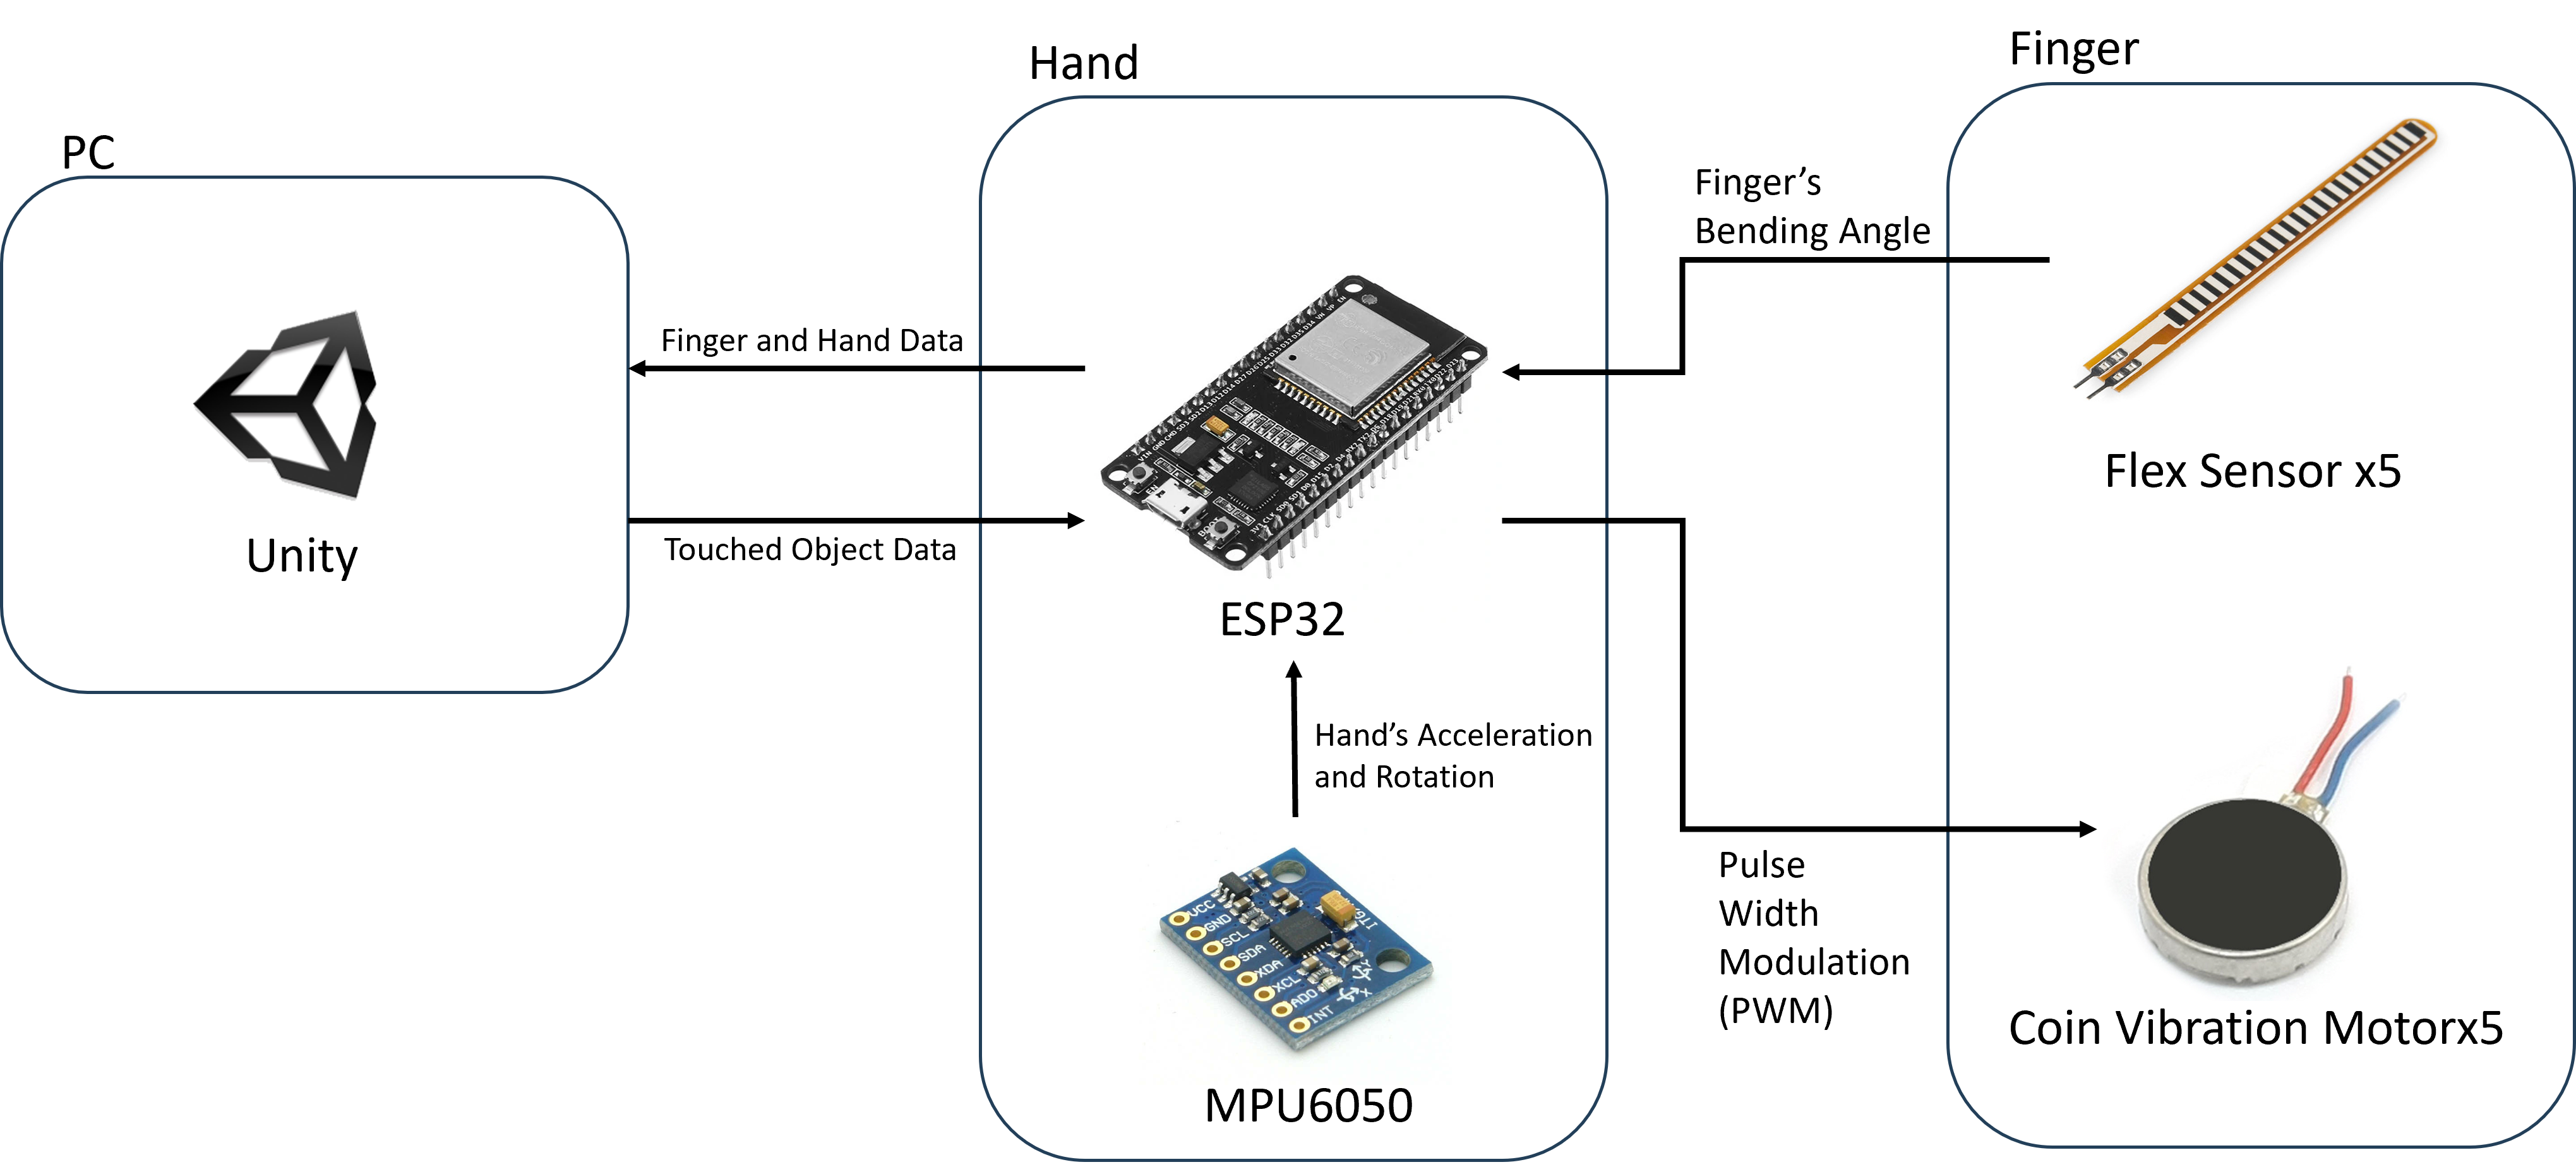
\includegraphics[width=1\textwidth]{figure/system diagram.png}%imagine Avation
	\caption{System architecture of the wearable haptic glove, showing integration between Unity, ESP32, and hardware components.}\label{fig:system_diagram}
\end{figure}
\textbf{ESP32 Microcontroller:}  
The ESP32 functions as the core processing unit, managing sensor data acquisition, real-time data processing, actuator control, and wireless communication. It employs Serial Communication to ensure continuous bidirectional data exchange with Unity, maintaining synchronization of haptic stimuli and sensor readings.

\textbf{Flex Sensors (x5):}  
Five resistive flex sensors, positioned along each finger of the glove, measure finger bending. These sensors deliver real-time analog signals corresponding to finger positions, enabling precise gesture recognition and accurate hand tracking.

\textbf{Inertial Measurement Unit (MPU-6050):}  
An MPU-6050 sensor captures spatial orientation, acceleration, and angular velocity data of hand movements. Integration of IMU measurements enhances spatial coherence between real and virtual hand positions, significantly improving immersive realism and spatial fidelity.

\textbf{Coin Vibration Motor:}  
A coin-type vibration motor generates controlled tactile feedback, utilizing Pulse Width Modulation (PWM) to replicate varying granularities in virtual textures. PWM modulation enables dynamic adjustment of vibration intensity and frequency, simulating realistic sensations from smooth to coarse surfaces. The device provides three distinct haptic feedback, systematically evaluating users' tactile perception sensitivity as recommended by prior research~\cite{strohmeier2017generating, bensmaia2003vibrations}.

The integration of these components into the wearable device is shown in Figure~\ref{fig:glove_1}.

\begin{figure}\centering
	\includegraphics[width=0.5\textwidth]{figure/glove_1.png}%imagine Avation
	\caption{Haptic Data Glove used for texture perception in virtual environments.}\label{fig:glove_1}
\end{figure}

This integrated approach facilitates intuitive interactions in virtual environments, enabling natural hand movements combined with realistic tactile sensations. The selected components directly address limitations noted in existing literature, achieving a lightweight, responsive design with nuanced texture rendering.

%%%%%%%%%%%%%%%%%%%%%%%%%%%%%%%%%%%%%%%%%%%%%%%%%%%%%%%%%%%%%%%%%%%%%%%%%
%%%%%%%%%%%%%%%%%%%%%%%%%%%%%%%%%%%%%%%%%%%%%%%%%%%%%%%%%%%%%%%%%%%%%%%%%
% Experiments
%%%%%%%%%%%%%%%%%%%%%%%%%%%%%%%%%%%%%%%%%%%%%%%%%%%%%%%%%%%%%%%%%%%%%%%%%
%%%%%%%%%%%%%%%%%%%%%%%%%%%%%%%%%%%%%%%%%%%%%%%%%%%%%%%%%%%%%%%%%%%%%%%%%
\section{Experiments}
We conducted two experiments to evaluate the effectiveness of the developed wearable haptic glove. Experiment~1 assessed participants' ability to differentiate among three distinct haptic feedback cycle rates, while Experiment~2 explored the relationship between these cycle rates and the perceived realism of different virtual textures.

Figure~\ref{fig:experiment_setup} shows the general experimental setup, highlighting participant interaction with the haptic glove in the virtual environment.

\begin{figure}\centering
	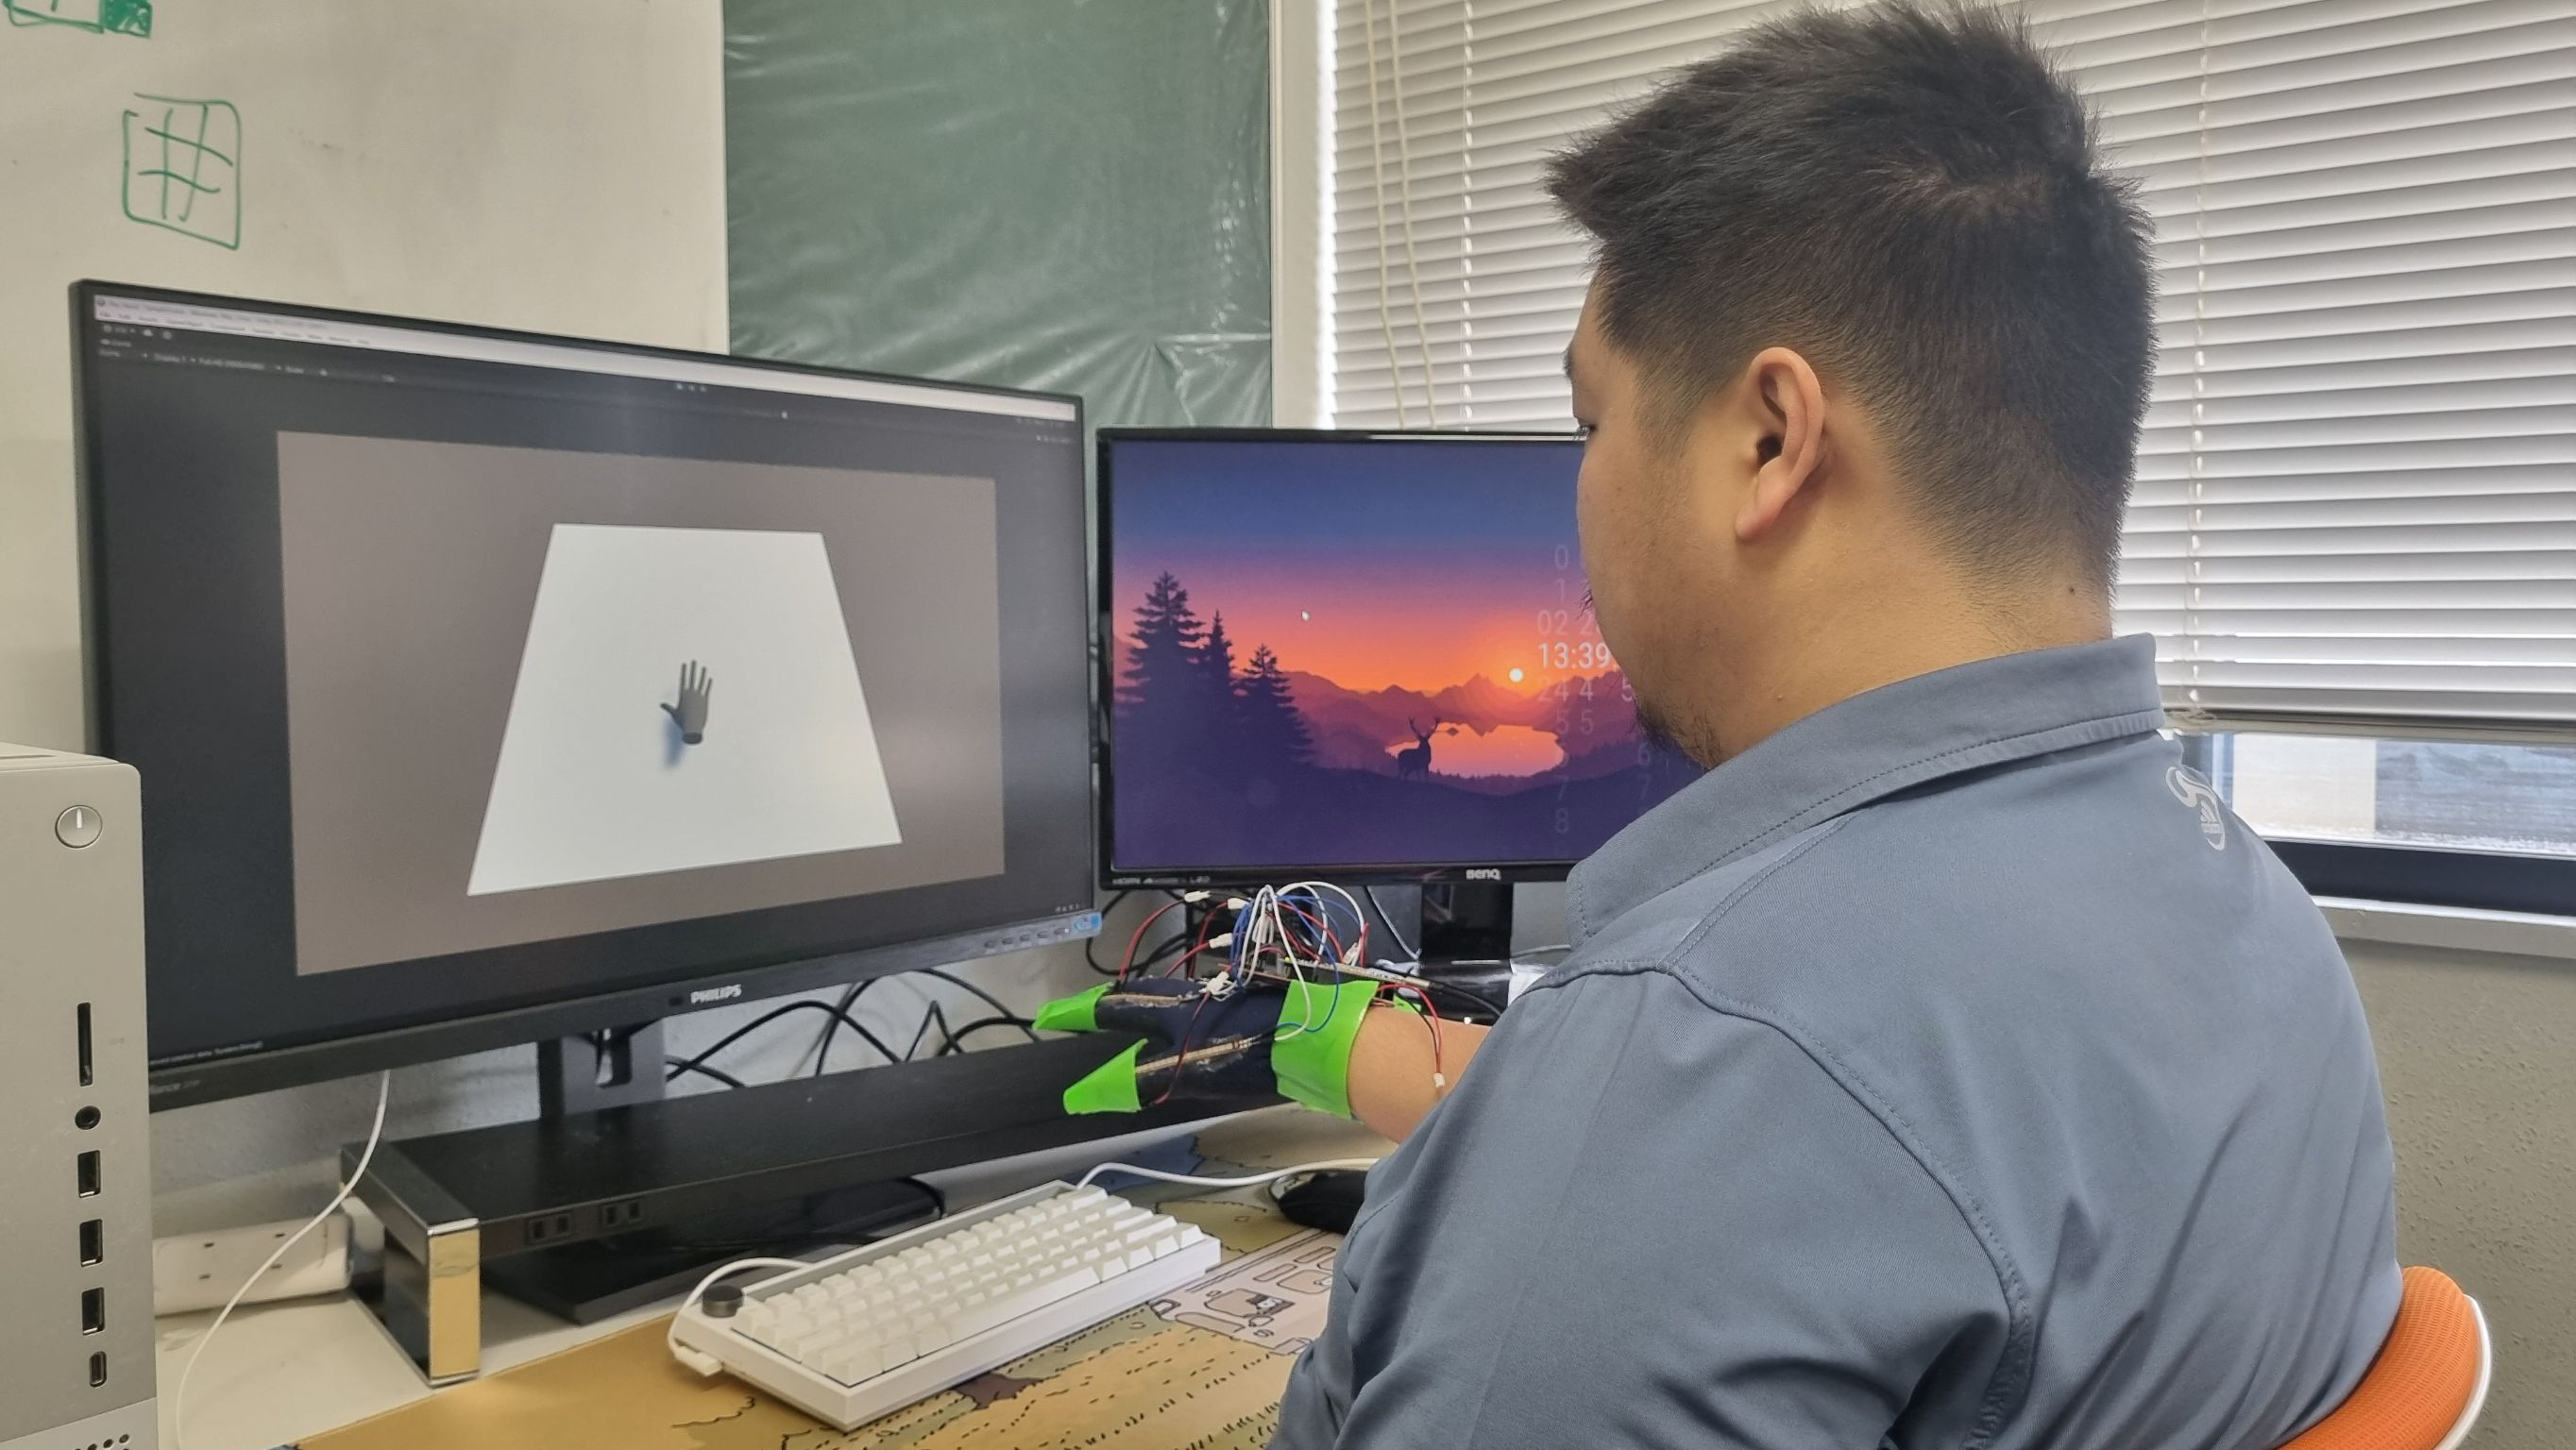
\includegraphics[width=0.7\textwidth]{figure/experiment.png}%imagine Avation
	\caption{Overall experimental setup demonstrating participant interaction using the wearable haptic glove.}\label{fig:experiment_setup}
\end{figure}

\subsection{Experiment 1: Distinguishing Haptic Feedback}
We recruited six participants aged 24–27 to performed a blind test to evaluate their ability to distinguish between three distinct vibration cycle rates: 0.2, 0.5, and 1.0. Before starting, participants were familiarized with each cycle rate to establish clear tactile references.
performed a blind test to evaluate their ability to distinguish between three distinct vibration cycle rates: 0.2, 0.5, and 1.0. Before starting, participants were familiarized with each cycle rate to establish clear tactile references.

\textbf{Procedure:} Participants wore and calibrated the glove through repeated hand opening and closing gestures, ensuring accurate hand tracking. Subsequently, participants interacted with a plain white 3D plane in the virtual environment (Figure~\ref{fig:experiment1_setup}), triggering randomly generated vibrations corresponding to one of the three cycle rates. Participants verbally identified the perceived cycle rate after each interaction. Each participant completed 15 randomized trials, assessing their discrimination accuracy.

\begin{figure}[H]
	\centering
	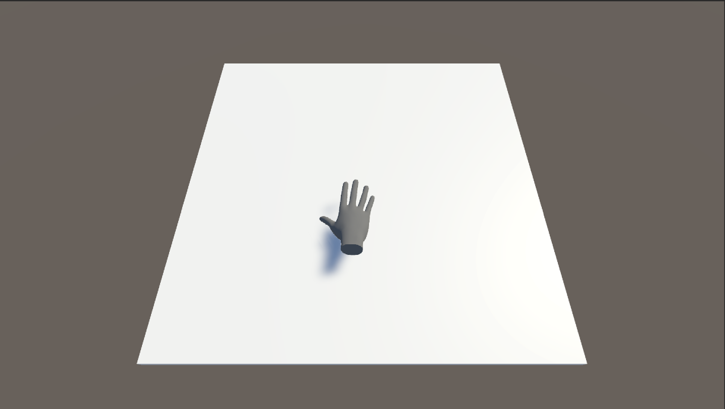
\includegraphics[width=0.7\textwidth]{figure/ex1.png}%imagine Avation
	\caption{Experimental setup for Experiment~1: participants interacting with a plain white virtual plane to distinguish vibration cycle rates.}\label{fig:experiment1_setup}
\end{figure}

\subsection{Experiment 2: Relationship Between Haptic Feedback and Texture Perception}
The participants from Experiment 1 were also involved in Experiment 2. This experiment explored how different vibration cycle rates influenced the perceived realism of virtual textures. Participants interacted with three visually distinct textures—brick, grass, and marble—each sequentially paired with vibration cycle rates of 0.2, 0.5, and 1.0.

\textbf{Procedure:} After the first experiment, participants took a 5-minute break before proceeding to the second experiment. In this phase, participants sequentially interacted with each virtual texture (Figure~\ref{fig:experiment2_setup}), experiencing all three vibration cycle rates (0.2, 0.5, and 1.0). After experiencing each set of cycle rates for a given texture, participants selected the cycle rate they felt most accurately matched the visual texture. This procedure was repeated for each texture type, with the order of textures presented randomly for each participant.

\begin{figure}\centering
	\includegraphics[width=1\textwidth]{figure/ex2.png}%imagine Avation
	\caption{Experimental setup for Experiment~2: participants interacting with textured virtual planes (brick, grass, marble) to assess vibration realism.}\label{fig:experiment2_setup}
\end{figure}

Collectively, these experiments provided insights into participants' perceptual sensitivity to different vibration cycle rates and evaluated the realism of tactile sensations corresponding to varied virtual textures.

\subsection{Post-Experiment Evaluation}
After completing both experiments, participants provided subjective feedback through a questionnaire consisting of 12 statements (Table~\ref{tab:evaluation_questions}). Each statement was rated on a Likert scale from 1 (strongly disagree) to 7 (strongly agree), covering virtual hand embodiment, tactile realism, and immersion. Questions about the sense of virtual hand ownership and control (e.g., Q1, Q3, Q4, Q8) were based on the Virtual Embodiment Questionnaire (VEQ)~\cite{roth2017alpha}. Statements assessing how realistic and aligned the tactile sensations felt (Q2, Q6, Q7, Q10) were guided by the Haptic Experience (HX) model~\cite{schneider2017haptic}. Additionally, overall immersion (Q12) was evaluated according to concepts from the Presence Questionnaire (PQ)~\cite{witmer1998measuring}.

\begin{table}[htbp]
    \centering
    \caption{Post-experiment evaluation questionnaire.}
    \label{tab:evaluation_questions}
    \resizebox{\textwidth}{!}{
    \begin{tabular}{c | c}
        \hline
        \textbf{Question} & \textbf{Statement}\\
        \hline
        Q1 & I felt as if the virtual hands were my own.\\\hline
        Q2 & I felt that the tactile sensations were caused by the virtual hand.\\\hline
        Q3 & I felt as if my hand were the virtual hand.\\\hline
        Q4 & I felt like I was controlling the movement of the virtual hand.\\\hline
        Q5 & I felt as if the virtual hand was naturally connected to my body.\\\hline
        Q6 & The tactile sensations I perceived felt naturally aligned with the virtual hand.\\\hline
        Q7 & When I touched the virtual plane, I felt as if my real hand was also being touched.\\\hline
        Q8 & The movements of the virtual hand felt natural to me.\\\hline
        Q9 & I felt that the virtual hand responded as expected to my movements.\\\hline
        Q10 & I had the sensation that I could feel the texture of objects through the virtual hand.\\\hline
        Q11 & I felt a mismatch between my real hand and the virtual hand.\\\hline
        Q12 & The overall experience made me feel immersed in the virtual environment.\\
        \hline
    \end{tabular}}
\end{table}

Participant responses provided qualitative insights into embodiment, tactile realism, and immersion, complementing the quantitative outcomes from Experiments~1 and 2.


%%%%%%%%%%%%%%%%%%%%%%%%%%%%%%%%%%%%%%%%%%%%%%%%%%%%%%%%%%%%%%%%%%%%%%%%%
%%%%%%%%%%%%%%%%%%%%%%%%%%%%%%%%%%%%%%%%%%%%%%%%%%%%%%%%%%%%%%%%%%%%%%%%%
% Results and Discussion
%%%%%%%%%%%%%%%%%%%%%%%%%%%%%%%%%%%%%%%%%%%%%%%%%%%%%%%%%%%%%%%%%%%%%%%%%
%%%%%%%%%%%%%%%%%%%%%%%%%%%%%%%%%%%%%%%%%%%%%%%%%%%%%%%%%%%%%%%%%%%%%%%%%

\section{Results and Discussion}

\subsection{Experiment 1: Distinguishing Haptic Feedback.}  

Participants' accuracy in identifying the three PWM cycle rates (0.2, 0.5, and 1.0) is summarized in Figure~\ref{fig:ex1_results}. The highest accuracy (26/30) was achieved at the 1.0 cycle rate, suggesting that participants found higher-intensity vibrations easier to identify. Accuracy slightly decreased at lower cycle rates (0.5: 24/30; 0.2: 23/30), indicating that subtler vibrations were more challenging to distinguish. This aligns with prior research indicating that higher vibration intensities yield clearer tactile distinctions~\cite{strohmeier2017generating,bensmaia2003vibrations}. These findings confirm the effectiveness of PWM cycle rates in distinguishing tactile sensations.

\begin{figure}\centering
	% 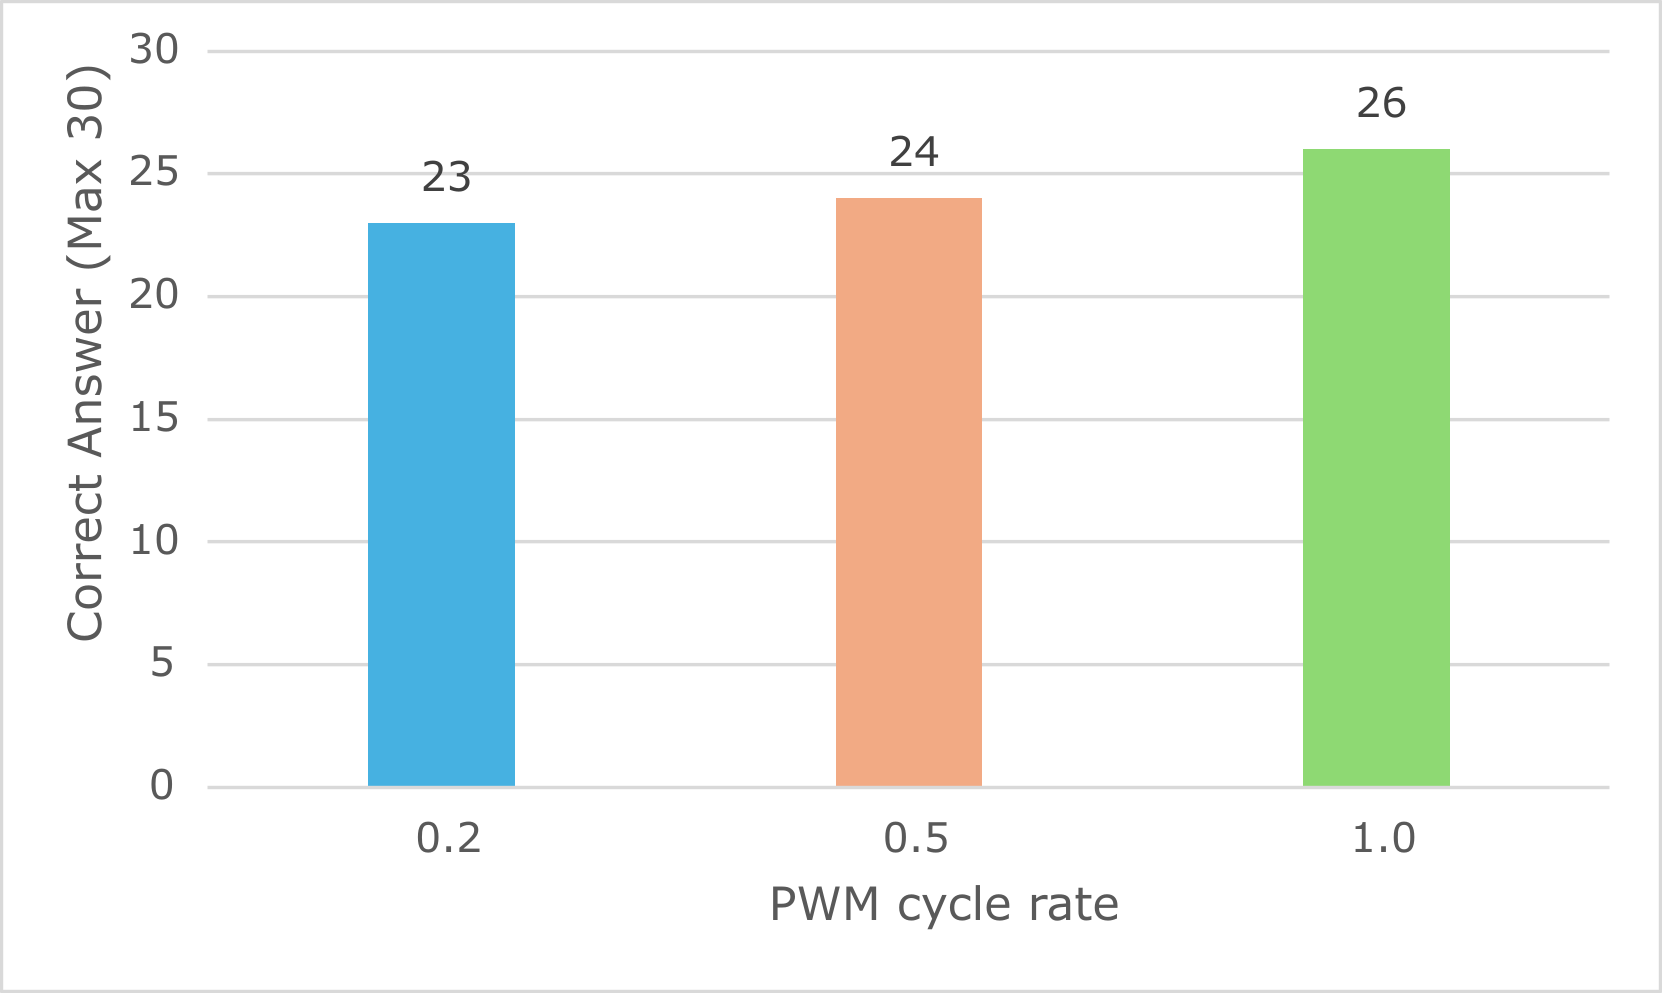
\includegraphics[width=0.8\textwidth]{figure/ex1_result.pdf}%imagine Avation
	\includesvg[width=0.7\textwidth, inkscapelatex=true]{figure/ex1_result}
	\caption{Participants' accuracy in identifying different vibration cycle rates.}\label{fig:ex1_results}
\end{figure}

\subsection{Experiment 2: Relationship Between Haptic Feedback and Texture Perception.}

Participants' preferences for associating specific vibration cycle rates with virtual textures (brick, grass, marble) are illustrated in Figure~\ref{fig:ex2_results}. The marble texture was unanimously associated with the highest cycle rate (1.0), suggesting participants perceived smoother and more rigid textures as best represented by higher-intensity vibrations. Conversely, the brick and grass textures elicited preferences for lower and intermediate cycle rates (0.2 and 0.5), reflecting participants' association of moderate vibrations with intermediate texture roughness. These results clearly highlight the link between vibration granularity and perceived realism, reinforcing the importance of tailored tactile feedback for different textures~\cite{otake2022vibrotactile}.

\begin{figure}[H]
	\centering
	% 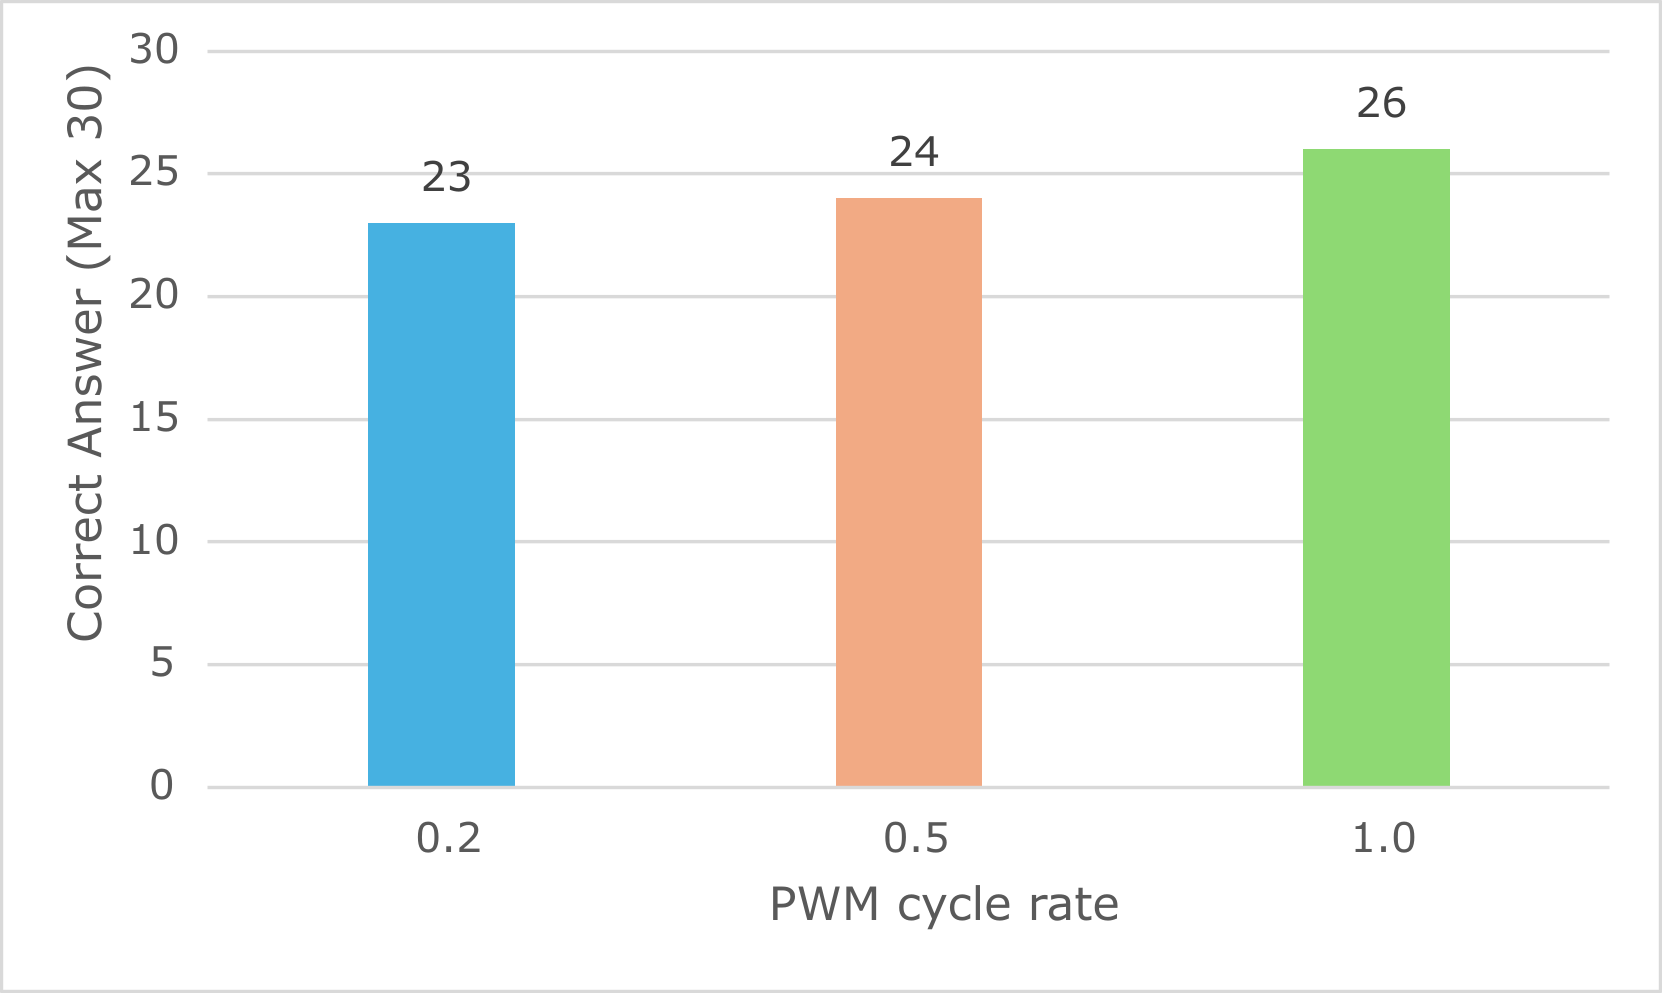
\includegraphics[width=0.8\textwidth]{figure/ex1_result.pdf}%imagine Avation
	\includesvg[width=0.7\textwidth, inkscapelatex=true]{figure/ex2_result}
	\caption{Participants' accuracy in identifying different vibration cycle rates.}\label{fig:ex2_results}
\end{figure}


\subsection{Post-Experiment Evaluation.} 

Subjective feedback (Figure~\ref{fig:questionnaire_results}) revealed high ratings in perceived texture realism (Q10; mean=5.33), tactile alignment (Q7; mean=5.00, Q6; mean=4.83), and overall immersion (Q12; mean=4.83). Moderate agreement was found in tactile sensations attributed directly to the virtual hand (Q2; mean=4.83) and control fidelity (Q4; mean=4.17). Lower scores in embodiment and naturalness of hand interactions (Q5; mean=3.17, Q8; mean=3.17) suggest areas needing further refinement. These results reinforce the success of the glove in enhancing tactile feedback realism and immersion, echoing findings from previous wearable haptic studies~\cite{pacchierotti2017wearable}. However, the lower embodiment scores indicate potential improvements in sensor placement or glove calibration procedures to strengthen the perceived naturalness of virtual hand interactions.

\begin{figure}\centering
	% 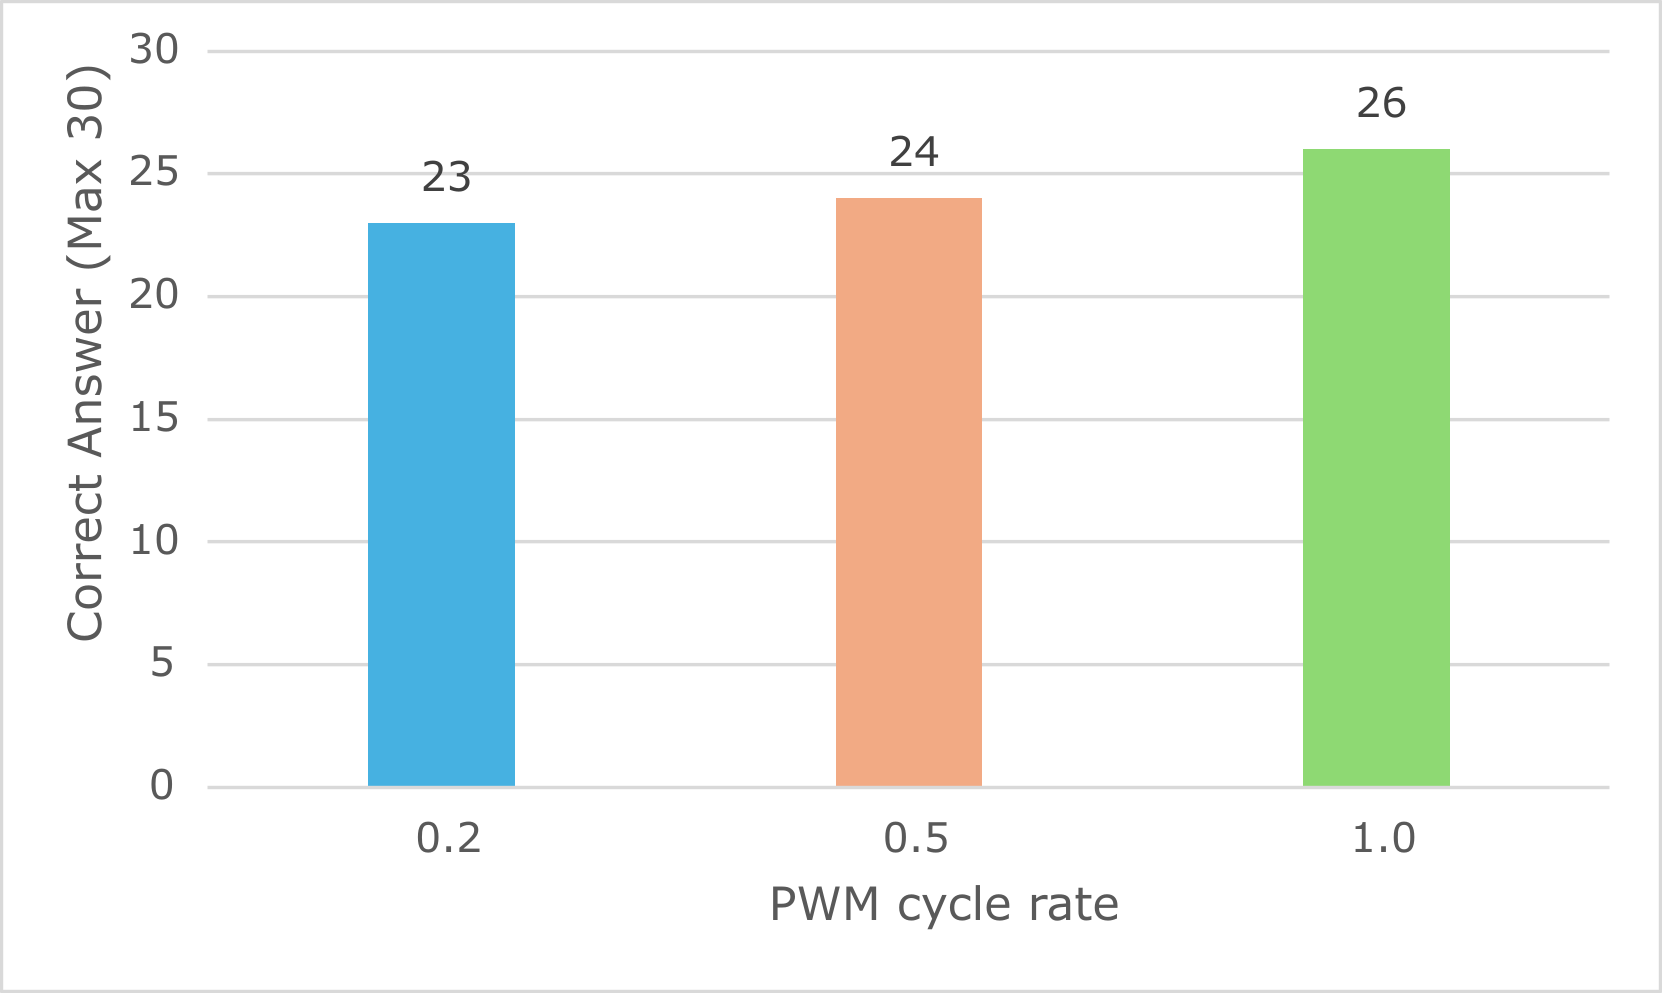
\includegraphics[width=0.8\textwidth]{figure/ex1_result.pdf}%imagine Avation
	\includesvg[width=0.7\textwidth, inkscapelatex=true]{figure/question_result}
	\caption{Participants' accuracy in identifying different vibration cycle rates.}\label{fig:questionnaire_results}
\end{figure}

\subsection{General Discussion.}  

Collectively, the experimental and subjective results demonstrate that PWM-based tactile feedback significantly improves users' ability to distinguish and realistically perceive virtual textures, contributing positively to overall immersion in virtual environments. The findings support previous literature emphasizing the importance of tactile granularity and frequency modulation for realistic texture rendering~\cite{strohmeier2017generating,bach2023enhanced}. Future iterations of the haptic glove should prioritize enhancing the sense of embodiment by refining hand tracking fidelity and further optimizing vibration characteristics for various textures.

%%%%%%%%%%%%%%%%%%%%%%%%%%%%%%%%%%%%%%%%%%%%%%%%%%%%%%%%%%%%%%%%%%%%%%%%%
%%%%%%%%%%%%%%%%%%%%%%%%%%%%%%%%%%%%%%%%%%%%%%%%%%%%%%%%%%%%%%%%%%%%%%%%%
% Conclusion and Future Work
%%%%%%%%%%%%%%%%%%%%%%%%%%%%%%%%%%%%%%%%%%%%%%%%%%%%%%%%%%%%%%%%%%%%%%%%%
%%%%%%%%%%%%%%%%%%%%%%%%%%%%%%%%%%%%%%%%%%%%%%%%%%%%%%%%%%%%%%%%%%%%%%%%%

\section{Conclusion and Future Work}

In this study, we developed a wearable haptic glove equipped with flex sensors, an IMU (MPU-6050), and a coin-type vibration motor to provide realistic tactile feedback in virtual environments. Two experiments were conducted to evaluate participants' ability to differentiate among various PWM-based vibration cycle rates and to explore how these tactile signals influenced their perception of virtual textures. The results indicated high accuracy in distinguishing vibration cycle rates, especially at higher intensities, and confirmed that specific cycle rates significantly enhanced the perceived realism of distinct virtual textures. Participants reported enhanced immersion, realistic tactile perception, and overall satisfaction with the haptic experience, although improvements in virtual embodiment were identified as necessary.

Future research will focus on improving the naturalness and embodiment aspects of virtual interactions by refining sensor placements, calibration methods, and incorporating additional haptic actuators for more nuanced tactile sensations. Furthermore, we aim to integrate adaptive feedback algorithms capable of dynamically adjusting vibration parameters based on real-time user interactions, further enhancing realism and immersive experiences within VR applications.


%\vspace{350cm}
%\begin{thebibliography}{10}
%\bibitem{Akyildiz}  
%Akyildiz  F.I., Wang X., Wang W.: Wireless Mesh Networks: A
%Survey. In: Computer Networks, Vol. 47, No. 4, pp. 445-487, 2005.

%\bibliographystyle{IEEEtran}
%\bibliographystyle{junsrt}		%出てきた順索引 
%\bibliographystyle{spbasic}
%\bibliographystyle{splncs04}
%\bibliographystyle{ieeetr}
\bibliographystyle{spmpsci}
%\bibliographystyle{splncs}

\bibliography{Ref}

\end{document}
